% !TeX TXS-program:compile = txs:///lualatex

\documentclass[a4paper,11pt]{article}
\usepackage[revgoku]{cp-base}
\graphicspath{{./graphics/}}
%variables
\donnees[%
	classe={1\up{ère} 2M2},matiere={[SPÉ.MATHS]},mois=Janvier,annee=2022,typedoc=CHAP,numdoc=6
]
%formatage
\author{Pierquet}
\title{\nomfichier}
\hypersetup{pdfauthor={Pierquet},pdftitle={\nomfichier},allbordercolors=white,pdfborder=0 0 0,pdfstartview=FitH}
%divers
\lhead{\entete{\matiere}}
\chead{\entete{\lycee}}
\rhead{\entete{\classe{} - \mois{} \annee}}
\lfoot{\pied{\matiere}}
\cfoot{\logolycee{}}
\rfoot{\pied{\numeropagetot}}

\begin{document}

\ifdef{\cercletrigo}{}{%
	\newcommand\cercletrigo{%
		\draw (0,0) circle[radius=2] ;
		\draw (-2.25,0) -- (2.25,0) ;
		\draw (0,-2.25) -- (0,2.25) ;
		\draw[->,>=stealth'] (0,0) -- (2,0) ;
		\draw[->,>=stealth'] (0,0) -- (0,2) ;
		\draw (0,0) node[below left] {$O$} ;}
}

\ifdef{\angl}{}{\newcommand\angl[2]{\dfrac{#1\pi}{#2}}}

\pagestyle{fancy}

\part{CH06 - Trigonométrie - Exercices}

\medskip

\begin{caide}
{\setlength\arrayrulewidth{1.5pt} \arrayrulecolor{titrebleu!35}
\begin{tabularx}{0.95\linewidth}{Y|Y|Y|Y|Y|Y}
	\niveaudif{0}~~\textsf{Basique} & \niveaudif{1}~~\textsf{Modérée} & \niveaudif{2}~~\textsf{Élevée} & \niveaudif{3}~~\textsf{Très élevée} & \niveaudif{4}~~\textsf{Extrême} & \niveaudif{5}~~\textsf{Insensée} \\
\end{tabularx}}
\end{caide}

\exonum{0}

\begin{enumerate}
	\item Convertir, en radians, les mesures données en degrés :\[\ang{10} \qquad ; \qquad \ang{59} \qquad ; \qquad \ang{180} \qquad ; \qquad \ang{18} \qquad ; \qquad \ang{72} \qquad ; \qquad \ang{112,5}.\]
	\item Convertir, en degrés, les mesures données en radians :\[ \dfrac{\pi}{3} \qquad ; \qquad \dfrac{2\pi}{3} \qquad ; \qquad \pi \qquad ; \qquad \dfrac{5\pi}{4} \qquad ; \qquad \dfrac{3\pi}{8} \qquad ; \qquad \dfrac{5\pi}{12} \qquad ; \qquad \dfrac{3\pi}{2}.\]
\end{enumerate}

\medskip

\exonum{1}

\medskip

Sur le cercle trigonométrique, placer les points images des angles en radians suivants :

\smallskip

\begin{minipage}{5cm}
	\begin{center}
		\begin{tikzpicture}[scale=0.66,very thick]]
			\cercletrigo
		\end{tikzpicture}
	\end{center}
\end{minipage}\hfill
\begin{minipage}{13cm}
	\begin{multicols}{4}
		\begin{enumerate}
			\item $\vphantom{\dfrac{3\pi}{4}}\pi$
			\item $\vphantom{\dfrac{3\pi}{4}}\dfrac{\pi}{4}$
			\item $\dfrac{3\pi}{2}$
			\item $\vphantom{\dfrac{3\pi}{4}}\dfrac{\pi}{6}$
			\item $\vphantom{\dfrac{3\pi}{4}}-\dfrac{\pi}{3}$
			\item $-\dfrac{3\pi}{4}$
			\item $\dfrac{5\pi}{6}$
			\item $-\dfrac{3\pi}{2}$
		\end{enumerate}
	\end{multicols}
\end{minipage}

\medskip

\exonum{2}

\medskip

On donne les figures suivantes :

\begin{center}
	\begin{center}
		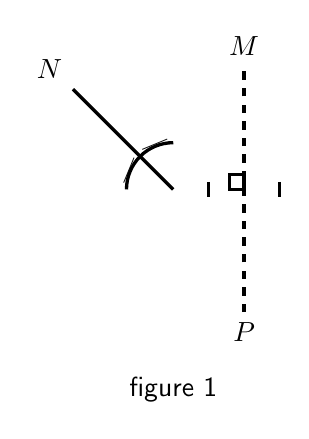
\begin{tikzpicture}[very thick,scale=0.9]
			\cercletrigo
			\draw[dashed] (-60:2) node[below] {$P$} -- (60:2) node[above] {$M$} ; 
			\draw (0.5,3pt) -- (0.5,-3pt) (1.5,3pt) -- (1.5,-3pt);
			\draw (1,0) rectangle ++ (-6pt,6pt) ;
			\draw (0,0) -- (135:2) node[above left] {$N$} ;
			\draw (0,0.66) arc(90:135:0.66) node[midway,sloped] {\footnotesize \bf |};
			\draw (135:0.66) arc(135:180:0.66) node[midway,sloped] {\footnotesize \bf |};
			\draw (0,-2.5) node[below] {\sffamily figure 1} ;
		\end{tikzpicture}
		\qquad\qquad\qquad
		\begin{tikzpicture}[very thick,scale=0.9]
			\cercletrigo
			\draw[dashed] (-150:2) node[left] {$R$} -- (-30:2) node[right] {$S$} ; 
			\draw (3pt,-0.5) -- (-3pt,-0.5) (3pt,-1.5) -- (-3pt,-1.5);
			\draw (0,-1) rectangle ++ (6pt,6pt) ;
			\draw (0.66,0) arc(0:45:0.66) node[midway,sloped] {\footnotesize \bf |};
			\draw (45:0.66) arc(45:90:0.66) node[midway,sloped] {\footnotesize \bf |};
			\draw (0,0) -- (45:2) node[above right] {$Q$} ;
			\draw (0,-2.5) node[below] {\sffamily figure 2} ;
		\end{tikzpicture}
	\end{center}
\end{center}

\begin{enumerate}
	\item Utiliser les informations de la {\sf figure 1} pour déterminer les angles, sur $\intervFO{0}{2\pi}$ repérant les points $M$, $N$ et $P$.
	\item Utiliser les informations de la {\sf figure 2} pour déterminer les angles, sur $\intervOF{-\pi}{\pi}$ repérant les points $Q$, $R$ et $S$.
\end{enumerate}

\medskip

\exonum{1}

\medskip

Dans chaque cas, trouver l'angle $x$ dans $\intervOF{-\pi}{\pi}$ (la mesure principale) correspondant à l'angle $\alpha$ donné :

\bigskip

\begin{minipage}{\linewidth}
	\begin{multicols}{5}
		\begin{enumerate}
			\item $\alpha = \angl{7}{2}$
			\item $\alpha = -\angl{4}{3}$
			\item $\alpha = \angl{35}{6}$
			\item $\alpha = -\angl{21}{4}$
			\item $\alpha = \angl{202}{3}$
		\end{enumerate}
	\end{multicols}
\end{minipage}

\newpage

\exonum{2}

\medskip

Trouver les valeurs exactes du cosinus, sinus puis de la tangente des réels donnés. (On pourra commencer par déterminer, si besoin, la mesure principale)

\begin{multicols}{5}
	\begin{enumerate}
		\item $\alpha=\vphantom{\angl{1}{2}}\angl{}{6}$
		\item $\alpha=\angl{5}{6}$
		\item $\alpha=\angl{7}{6}$
		\item $\alpha=\angl{11}{6}$
		\item $\alpha=\angl{13}{6}$
	\end{enumerate}
\end{multicols}
\begin{multicols}{5}
	\begin{enumerate}\addtocounter{enumi}{5}
		\item $\alpha=\vphantom{\angl{1}{2}}\angl{}{4}$
		\item $\alpha=\angl{9}{4}$
		\item $\alpha=\angl{5}{4}$
		\item $\alpha=\angl{81}{4}$
		\item $\alpha=-\angl{108}{4}$
	\end{enumerate}
\end{multicols}
\begin{multicols}{5}
	\begin{enumerate}\addtocounter{enumi}{10}
		\item $\alpha=\angl{4}{3}$
		\item $\alpha=\vphantom{\angl{1}{2}}\angl{}{3}$
		\item $\alpha=\angl{71}{3}$
		\item $\alpha=\angl{97}{3}$
		\item $\alpha=-\angl{54}{3}$
	\end{enumerate}
\end{multicols}

\medskip

\exonum{2}

\medskip

Sur le cercle trigonométrique colorier les arcs décrits par les intervalles $\mathscr{I}$, $\mathscr{J}$ et $\mathscr{K}$ tels que : \[ \mathscr{I}=\intervFF{-\dfrac{\pi}{4}}{\dfrac{5\pi}{4}} \qquad ; \qquad \mathscr{J}=\intervFF{\dfrac{4\pi}{3}}{\dfrac{13\pi}{6}} \qquad ; \qquad \mathscr{K}=\intervFF{-\dfrac{7\pi}{6}}{\dfrac{5\pi}{4}}. \]
\begin{center}
	\begin{tikzpicture}[very thick,scale=0.66]
		\cercletrigo
	\end{tikzpicture}
	\qquad \qquad
	\begin{tikzpicture}[very thick,scale=0.66]
		\cercletrigo
	\end{tikzpicture}
	\qquad \qquad
	\begin{tikzpicture}[very thick,scale=0.66]
		\cercletrigo
	\end{tikzpicture}
\end{center}

\medskip

\exonum{2}

\medskip

À l’aide d’un cercle trigonométrique, résoudre dans $\R$ les équations suivantes :
\begin{multicols}{3}
	\begin{enumerate}
		\item $\cos(x)=\dfrac{\sqrt{2}}{2}$ ;
		\item $\sin(x)=0\vphantom{\dfrac{\sqrt{2}}{2}}$ ;
		\item $2\sin(x)+\sqrt{3}=0\vphantom{\dfrac{\sqrt{2}}{2}}$.
	\end{enumerate}
\end{multicols}

\medskip

\exonum{3}

\begin{enumerate}
	\item À l’aide de la formule $\sin^2(x) +\cos^2(x) =1$ :
	\begin{enumerate}
		\item déterminer $\cos(x)$ sachant que : $\sin(x)=\dfrac23$ et $x \in \intervFF{0}{\dfrac{\pi}{2}}$ ;
		\item déterminer $\sin(x)$ sachant que : $\cos(x)=-\dfrac15$ et $x \in \intervFF{-\pi}{0}$ ;
		\item déterminer $\cos(x)$ sachant que : $\sin(x)=-\dfrac{\sqrt{5}}{3}$ et $x \in \intervFF{\dfrac{\pi}{2}}{\pi}$.
	\end{enumerate}
	\item Démontrer que pour tout réel $x$ on a :
	\begin{enumerate}
		\item $\big(\cos(x) + \sin(x)\big)^2 + \big(\cos(x) - \sin(x)\big)^2 = 2$ ;
		\item $\big(\cos(x) + \sin(x)\big)^2 - \big(\cos(x) - \sin(x)\big)^2 = 4\cos(x)\sin(x)$.
	\end{enumerate}
%	\item Exprimer à l’aide de $\sin(x)$ et $\cos(x)$, les expressions suivantes :
%	\begin{enumerate}
%		\item $\sin(-x) + \cos(-x)$ ;
%		\item $\sin(-x) - \sin(\pi +x)$ ;
%		\item $\sin(-x) + \cos(-x)$ ;
%		\item $\sin\left(x+\angl{}{2}\right) - 3\cos \left(-\angl{}{2} - x \right) - 4 \sin(\pi-x)$.
%	\end{enumerate}
\end{enumerate}

\medskip

\exonum{4}

\medskip

Résoudre dans $\R$ puis visualiser les solutions dans le cercle trigonométrique des équations suivantes :
\begin{enumerate}
	\item $2\sin \left(x+\angl{}{4}\right)-1 = 0$ ;
	\item $1-\sqrt{2} \cos \left(\angl{}{3} - x \right) = 0$ ;
	\item $\sin \left(2x - \angl{}{4} \right) = \dfrac12$ ;
	\item $\cos \left(2x -\angl{}{3} \right) = \dfrac12$.
\end{enumerate}

\end{document}